% This work is licensed under the Creative Commons Attribution-NonCommercial-ShareAlike 3.0 Unported License.
% To view a copy of this license, visit http://creativecommons.org/licenses/by-nc-sa/3.0/ or send a letter to 
% Creative Commons, 444 Castro Street, Suite 900, Mountain View, California, 94041, USA.

\documentclass[10pt]{article}
\usepackage{times}
\usepackage{latexsym}
\usepackage{graphicx}
\usepackage{amsmath, amsthm, amssymb}
\usepackage{nicefrac}
\usepackage{xspace}
\usepackage{appendix}
\usepackage{url}

% Use more of the page
\setlength{\topmargin}{0.0in}
\setlength{\textheight}{9.0in}

% Gives equations room in which to expand on the right
% \addtolength{\oddsidemargin}{-1.0in}

% Various shorthands for mathmode
\newcommand{\bs}[1]{\boldsymbol{#1}}
\newcommand{\mc}[1]{\mathcal{#1}}
\newcommand{\rl}[1]{\mathbb{R}^{#1}}

\newcommand{\argmax}[1]{\underset{#1}{\operatorname{argmax}\:}}
\newcommand{\argmin}[1]{\underset{#1}{\operatorname{argmin}\:}}
\newcommand{\mmax}[1]{\underset{#1}{\max\:}}
\newcommand{\mmin}[1]{\underset{#1}{\min\:}}

\newcommand{\vecop}[1]{\operatorname{vec}\left( #1 \right)}
\newcommand{\tinyurl}[1]{\tiny{\url{#1}}}

\newcommand{\norm}[1]{\mathcal{N}\left( #1 \right)}
\newcommand{\pd}[2]{\frac{\partial #1}{\partial #2}}
\newcommand{\logp}[1]{\log\left( #1 \right)}
\newcommand{\lnp}[1]{\ln\left( #1 \right)}
\newcommand{\expp}[1]{\exp\left( #1 \right)}
\newcommand{\abs}[1]{\left| #1 \right|}
\DeclareMathOperator{\sgn}{sgn}

% Ordinal superscripts; these should work in normal or mathmode
\newcommand{\superscript}[1]{\ensuremath{^{\textrm{#1}}} }
\newcommand{\subscript}[1]{\ensuremath{_{\textrm{#1}}} }
\newcommand{\xth}[0]{\superscript{th}}
\newcommand{\xst}[0]{\superscript{st}}
\newcommand{\xnd}[0]{\superscript{nd}}
\newcommand{\xrd}[0]{\superscript{rd}}

\newcommand{\ngram}{$n$-gram\xspace}
\newcommand{\ngrams}{$n$-grams\xspace}
\newcommand{\Ngram}{$N$-gram\xspace}
\newcommand{\Ngrams}{$N$-grams\xspace}
\newcommand{\BNgram}{$\mathbf{N}$-gram\xspace}
\newcommand{\BNgrams}{$\mathbf{N}$-grams\xspace}

\newcommand{\bgram}{($n$-1)-gram\xspace}
\newcommand{\bgrams}{($n$-1)-grams\xspace}
\newcommand{\Bgram}{($N$-1)-gram\xspace}
\newcommand{\Bgrams}{($N$-1)-grams\xspace}

\newcommand{\cnt}[1]{\mathfrak{C}\left(#1\right)}
\newcommand{\prb}[1]{P\left(#1\right)}
\newcommand{\cprb}[2]{P\left(#1 \;\middle\vert\; #2 \right)}
\newcommand{\hprb}[1]{\widehat{P}\left(#1\right)}
\newcommand{\hcprb}[2]{\widehat{P}\left(#1  \;\middle\vert\; #2 \right)}

\begin{document}

\title{Modified Kneser-Ney Language Modeling}

\author{Brian Romanowski\\
btr@msu.edu} 
\date{February 26, 2011}

\maketitle

%%%%%%%%%%%%%%%%%%%%%%%%%%%%%%%%%%%%%%%%%%%%%%
% Code fragments
%%%%%%%%%%%%%%%%%%%%%%%%%%%%%%%%%%%%%%%%%%%%%%

% \begin{figure}[h!]
% \centering
% \includegraphics[scale=0.60]{lassoWeights.loose.noOffset.eps}
% \caption{Weights $\beta$ for lasso regression as $\lambda$ varies.}
% \label{lassoWeights}
% \end{figure}

% \begin{table}[h!]
% \begin{center}
% \begin{tabular}{| l || c | c | c | }
% \hline
% $\lambda$ & training & validating & testing \\ \hline
% \end{tabular}
% \caption{Logistic regression accuracy on the heartstatlog corpus, averaged accuracy across 5 folds of the training data}
% \label{p1results}
% \end{center}
% \end{table}


% \begin{abstract}
% \end{abstract}

%%%%%%%%%%%%%%%%%%%%%%%%%%%%%%%%%%%%%%%%%%%%%%%%%%%%%%%%%%%%%%%%%%%%%%%%%%%%%%
%%%%%%%%%%%%%%%%%%%%%%%%%%%%%%%%%%%%%%%%%%%%%%%%%%%%%%%%%%%%%%%%%%%%%%%%%%%%%%
%%%%%%%%%%%%%%%%%%%%%%%%%%%%%%%%%%%%%%%%%%%%%%%%%%%%%%%%%%%%%%%%%%%%%%%%%%%%%%
\section{Introduction}
Statistical language models are a convenient way to capture linguistic information for use in automated systems.
They assign a probability to a sequence of words such that common/expected word sequences have higher associated probability than uncommon/unexpected sequences.
Estimating\footnote{I would say statistical language models $\subset$ probabalistic language models; they both report probabilities, but statistical language model parameters are necessarily based on statistical estimates from some training data} these probabilities from training data allows for good performance in new domains with minimum human intervention.
Language models are often combined with other sources of information to improve performance in applications like automated speech recognition, machine translation, and spell checking.

This report describes one particular language modeling technique in detail: the simpler version of Chen and Goodman's modified Kneser-Ney \ngram language model \cite{chen1998empirical}.
Supporting sections describe the mathematical notation, language modeling background, and the evaluation of language models.


%%%%%%%%%%%%%%%%%%%%%%%%%%%%%%%%%%%%%%%%%%%%%%%%%%%%%%%%%%%%%%%%%%%%%%%%%%%%%%
%%%%%%%%%%%%%%%%%%%%%%%%%%%%%%%%%%%%%%%%%%%%%%%%%%%%%%%%%%%%%%%%%%%%%%%%%%%%%%
%%%%%%%%%%%%%%%%%%%%%%%%%%%%%%%%%%%%%%%%%%%%%%%%%%%%%%%%%%%%%%%%%%%%%%%%%%%%%%
\section{Notation} 

Let $w_t$ indicate the word at index $t$ in some sequence of $n$ words $w_1^n$ chosen from a vocabulary $V$.
The subsequence starting with the word $w_i$ and ending with the word $w_j$, inclusive, is denoted by $w_i^j$.
Alternatively, a subsequence of $n$ words that ends at word $w_j$ is denoted by $w^j_{j-(n-1)}$.
This notation is illustrated in figure~\ref{figNotation}.
\begin{figure}[h!]
\centering
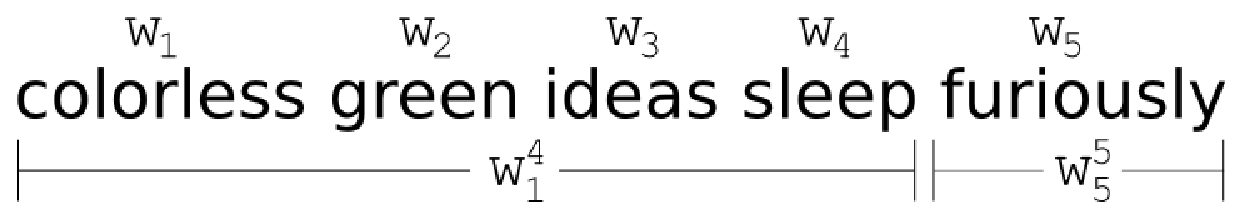
\includegraphics[scale=0.40]{notation.eps}
\caption{Indexing notation}
\label{figNotation}
\end{figure}

The probability of a sequence of $n$ words $v',v'',\ldots,v^{\prime\prime\cdots\prime}$ is denoted by:
\begin{align}
\prb{\bs{w^j_{j-(n-1)}} {=} v',v'',\ldots,v^{\prime\prime\cdots\prime}} &= \prb{\bs{w_{j-(n-1)}}{=}v',\bs{w_{j-(n-2)}}{=}v'',\ldots,\bs{w_j}{=}v^{\prime\prime\cdots\prime}} \label{equProbWordsStrict}
\end{align}
In this expression, each $\bs{w_t}$ is a categorically distributed random variable with possible outcomes being the finite set of vocabulary words $v \in V$.

When the actual word sequence is clear from context or when we make statements about the probability of a generalized word sequence, this simpler notation is used:
\begin{align}
\prb{w^j_{j-(n-1)}} &= \prb{w_{j-(n-1)},w_{j-(n-2)},\ldots,w_j} \label{equProbWords}
\end{align}

The conditional probability of the word at position $w_j$ given the previous $n-1$ word history is used extensively in language modeling:
\begin{align}
\cprb{w_j}{w^{j-1}_{j-(n-1)}} = \frac{ \prb{w^{j}_{j-(n-1)}} }{ \prb{w^{j-1}_{j-(n-1)}} }
\end{align}
When the conditional probability depends upon words at index $j < 1$, such as at the start of a document, generic ``words'' that serve to mark the start of the document are assumed/faked/inserted.

Counts of word sequences are often used to produce probability estimates like those above.
The counting function $\cnt{\cdot}$ counts the number of times word sequences occur, such that:
\begin{align}
\cnt{w_i^j} = d
\end{align}
is defined to mean that the word sequence $w_i^j$ occurred $d$ times in some sample of text.

The Kneser-Ney family of language model smoothing techniques make use of an additional quantity:
\begin{align}
N_i(w^{j-1}_{j-(n-1)}\bullet) = \text{\# unique words that follow $w^{j-1}_{j-(n-1)}$ exactly $i$ times} 
\end{align}
The notation $N_{i+}$ indicates the number of unique words that follow the word sequence at least $i$ times.


%%%%%%%%%%%%%%%%%%%%%%%%%%%%%%%%%%%%%%%%%%%%%%%%%%%%%%%%%%%%%%%%%%%%%%%%%%%%%%
%%%%%%%%%%%%%%%%%%%%%%%%%%%%%%%%%%%%%%%%%%%%%%%%%%%%%%%%%%%%%%%%%%%%%%%%%%%%%%
%%%%%%%%%%%%%%%%%%%%%%%%%%%%%%%%%%%%%%%%%%%%%%%%%%%%%%%%%%%%%%%%%%%%%%%%%%%%%%
\section{\BNgram Language Models}
A straightforward way to estimate the probability of a word sequence is to use the maximum likelihood 
estimator\footnote{This is the maximum likelihood estimator for a multinomial distribution over conditionally independent categorical events.  It is analogous to the maximum likelihood estimator for a binomial distribution over a sequence of Bernoulli random variables.}:
\begin{align}
\hprb{w_i^j} &= \frac{\cnt{w_i^j}}{N} \label{equSeqFreq}
\end{align}

If the word sequence $w_i^j$ is relatively long (say six words) compared to the amount of training data that is available (say one billion words of web data), we will not find many occurrences of $w_i^j$ in the training data.
For sequences that occur infrequently, the maximum likelihood estimate $\hprb{w_i^j}$ is not reliable, and will often be a poor estimate of the true probability $\prb{w_i^j}$.

One step towards a solution is to make the word sequences short, so that they are more likely to occur often in training data.
To accomplish this process, we first decompose the probability of a sequence of words according to the chain rule of probability:
\begin{align}
\prb{w_i^j} &= \prb{w_i^{j-1}} \cdot \cprb{w_j}{w_i^{j-1}}   \nonumber \\
&= \prb{w_i} \cdot \cprb{w_{i+1}}{w_i} \cdots \cprb{w_{j-1}}{w_i^{j-2}} \cdot \cprb{w_j}{w_i^{j-1}} \label{equChainRule} 
\end{align}

If we assume that the each word $w_j$ is only dependent on the previous $n-1$ words, equation~\ref{equChainRule} simplifies to the following:
\begin{align}
\prb{w_i^j} &\approx \cprb{w_j}{w_{j-(n-1)}^{j-1}} \cdot \cprb{w_{j-1}}{w_{j-(n-1)}^{j-2}} \cdots \cprb{w_{i+1}}{w_i} \cdot \prb{w_i} \label{equNGram}
\end{align}
This is the \emph{\ngram assumption}.
% It is false, as indicated in \cite{rosenfeld1995maximum} (discussed below), but it works relatively well in practice \cite{shannon1948mathematical}.

In an \ngram model, the probability of the $n\xth$ word depends only upon the $n-1$ previous words.
Each of these conditional probability distributions (i.e., model parameters) may be estimated by the relative frequency calculation:
\begin{align}
\hcprb{w_j}{w^{j-1}_{j-(n-1)}} &= \frac{\hprb{w^{j}_{j-(n-1)}}}{\hprb{w^{j-1}_{j-(n-1)}}} \\
&= \frac{\nicefrac{\cnt{w^{j}_{j-(n-1)}}}{N}}{\nicefrac{\cnt{w^{j-1}_{j-(n-1)}}}{N}} \\
&= \frac{\cnt{w^{j}_{j-(n-1)}}}{\cnt{w^{j-1}_{j-(n-1)}}} \label{equSeqFreq} %\\
% &= \frac{\cnt{w^{j}_{j-(n-1)}}}{\sum_{w_j} \cnt{w^{j}_{j-(n-1)}}} \label{equMargSeqFreq}
\end{align}
% Where in equation~\ref{equMargSeqFreq}, the count of the preceding $n-1$ length word history is obtained by marginalizing over the $n\xth$ word.

\Ngram models are often referred to with Latin prefixes for low order \ngrams and with numeral prefixes for high order \ngrams as: unigram, bigram, trigram, $4$-gram, $5$-gram, etc.


%%%%%%%%%%%%%%%%%%%%%%%%%%%%%%%%%%%%%%%%%%%%%%%%%%%%%%%%%%%%%%%%%%%%%%%%%%%%%%
%%%%%%%%%%%%%%%%%%%%%%%%%%%%%%%%%%%%%%%%%%%%%%%%%%%%%%%%%%%%%%%%%%%%%%%%%%%%%%
%%%%%%%%%%%%%%%%%%%%%%%%%%%%%%%%%%%%%%%%%%%%%%%%%%%%%%%%%%%%%%%%%%%%%%%%%%%%%%
\section{The Problem of Sparsity}
The \ngram assumption helps mitigate sparsity problems, but there are still many word sequences that are seen rarely or not at all in training data.
The worst case occurs when there is a sequence of words encountered during testing that was not encountered during training.

As an example, consider a bigram model is trained on the Brown corpus.
Suppose the model is used to calculate the probability of the sentence: ``the quick brown fox''.
\begin{align}
\prb{w_1^4} &= P(\text{``the''}) P(\text{``quick''$|$``the''}) P(\text{``brown''$|$``quick''}) P(\text{``fox''$|$``brown''}) \label{equSomeBigram}
\end{align}

It is reasonable that all of these bigrams will appear in a large training corpus and will have non-zero probabilities.
However, it may be the case that some bigrams in the similar sentence ``the quick \emph{wily} fox'' will \emph{not} appear in training 
data.\footnote{All bigrams in \ref{equSomeBigram} appear at least 100,000 times in reported Google search results, whereas the bigram ``quick wily'' appears in only 500 reported Google search results.}

If the bigram ``quick wily'' was not seen in the training data, its relative frequency estimate is zero.
\begin{align}
\prb{w_1^4} &= P(\text{``the''}) P(\text{``quick''$|$``the''}) P(\text{``wily''$|$``quick''}) P(\text{``fox''$|$``wily''}) \label{equZeroBigram} \\
&= P(\text{``the''}) P(\text{``quick''$|$``the''}) \cdot \bs{0} \cdot P(\text{``fox''$|$``wily''}) \\
&= \bs{0}
\end{align}
The presence of just one unseen bigram can prevent consideration of a syntactically and semantically valid sentence.


%%%%%%%%%%%%%%%%%%%%%%%%%%%%%%%%%%%%%%%%%%%%%%%%%%%%%%%%%%%%%%%%%%%%%%%%%%%%%%
%%%%%%%%%%%%%%%%%%%%%%%%%%%%%%%%%%%%%%%%%%%%%%%%%%%%%%%%%%%%%%%%%%%%%%%%%%%%%%
%%%%%%%%%%%%%%%%%%%%%%%%%%%%%%%%%%%%%%%%%%%%%%%%%%%%%%%%%%%%%%%%%%%%%%%%%%%%%%
\section{Modified Kneser-Ney Smoothing}
Kneser-Ney smoothing \cite{kneser1995improved} was modified slightly by Chen and Goodman \cite{chen1998empirical}.
Below is a description of the simpler version of their algorithm; the more complicated version that optimizes parameter values on held-out data is not discussed.

The modified Kneser-Ney smoothing relation is defined recursively as follows:
\begin{align}
\hcprb{w_j}{w^{j-1}_{j-(n-1)}} &= \frac{ \cnt{w^{j}_{j-(n-1)}} - D_n\left( \cnt{w^{j}_{j-(n-1)}} \right)}{ \sum_{w_j} \cnt{w^{j-1}_{j-(n-1)},w_j} } + \gamma\left( w^{j-1}_{j-(n-1)} \right) \hcprb{w_j}{w^{j-1}_{j-(n-2)}}
\end{align}
where
\begin{align}
D_n(c) =
  \begin{cases}
  0 & \text{if } c=0 \\
  1 - 2\left(\frac{n_1}{n_1+2n_2}\right)\left(\frac{n_2}{n_1}\right) & \text{if } c=1 \\
  2 - 3\left(\frac{n_1}{n_1+2n_2}\right)\left(\frac{n_3}{n_2}\right) & \text{if } c=2 \\
  3 - 4\left(\frac{n_1}{n_1+2n_2}\right)\left(\frac{n_4}{n_3}\right) & \text{if } c\geq 3 \text{ indicated by ``$c=3+$''}
  \end{cases}
\end{align}
where $n_i$ are the number of \ngrams of order $n$ that appear $i$ times in the training data, and:
\begin{align}
\gamma\left(w^{j-1}_{j-(n-1)}\right) = \frac{D_n(1)N_1\left(w^{j-1}_{j-(n-1)}\bullet\right) + D_n(2)N_2\left(w^{j-1}_{j-(n-1)}\bullet\right) + D_n(3+)N_{3+}\left(w^{j-1}_{j-(n-1)}\bullet\right)}{\sum_{w_j} \cnt{w^{j-1}_{j-(n-1)},w_j}}
\end{align}
We assume a closed vocabulary and terminate the recursion such that the unigram probability is just the maximum likelihood estimate:
\begin{align}
\hprb{w_j} = \frac{\cnt{w_j}}{N}
\end{align}

These equations are all taken directly from the Chen and Goodman paper; however, we make explicit the fact that the parameters $D_n(c)$ are calculated for each order $n$.

Things to prove or examine (most of these things are proven in Chen and Goodman):
\begin{itemize}
\item $\sum_{w_j} \hcprb{w_j}{w^{j-1}_{j-(n-1)}} = 1$
\item intution of $\gamma(\cdot)$
\item intuition behind KN
\item Is this generally how SRILM does it?
\end{itemize}

%%%%%%%%%%%%%%%%%%%%%%%%%%%%%%%%%%%%%%%%%%%%%%%%%%%%%%%%%%%%%%%%%%%%%%%%%%%%%%
%%%%%%%%%%%%%%%%%%%%%%%%%%%%%%%%%%%%%%%%%%%%%%%%%%%%%%%%%%%%%%%%%%%%%%%%%%%%%%
%%%%%%%%%%%%%%%%%%%%%%%%%%%%%%%%%%%%%%%%%%%%%%%%%%%%%%%%%%%%%%%%%%%%%%%%%%%%%%
\section{Evaluation}
For a particular task, language model performance is best modeled by using a language model as a component \emph{in situ}, in a full system.
In this setup, the language model may effect system accuracy, but may also be analyzed with respect to training time, model size, and performance as the task domain changes in time.
However, the necessity of repeated system runs and the difficulty of collecting adequate test data can make \emph{in situ} evaluations costly. 
Additionally, it is not obvious how performance results conditioned on a particular task informs the \emph{in situ} performance in a different task or domain.


%%%%%%%%%%%%%%%%%%%%
%%%%%%%%%%%%%%%%%%%%
\subsection{Perplexity}

The \emph{perplexity} metric measures language model performance with respect to textual testing data.
Language model perplexity is often strongly correlated with task performance.
Perplexity may be defined as shown \cite{jurafsky2008speech}:
\begin{align}
\text{PP}(W) = \prb{w_1^N}^{- \frac{1}{N}}
\end{align}
where $\text{PP}(W)$ is the perplexity of a test data set $w_1^N$.

This definition of perplexity may be interpreted as the geometric mean of the inverse probability of the test set.
The probability of the test data is a product of $N$ individual conditional \ngram probabilities.
The geometric mean is the number that, when multiplied $N$ times, produces an equivalent probability.
This value characterizes the average uncertainty of a word in the testing data.

The perplexity, as the inverse of the geometric mean, can be viewed as average size of the set of equiprobable words at each index in the test dataset.
Thus, \emph{lower perplexity indicates a better fitting model}, because there is a smaller number of word alternatives for each word in the testing data, on average.

Perplexity is also related to the information theoretic quantity \emph{cross entropy}.
See appendix~\ref{appendixPerplexity} for the proof that perplexity is related to cross entropy in the following manner:
\begin{align}
H(p,q) &= \lg \text{PP}(w_1^N) \label{equCrossEntropyPerplexity}
\end{align}
where $H(\cdot,\cdot)$ is cross entropy and $\lg$ is the base $2$ logarithm. 

Improvements in perplexity do not always correspond to improvements in task performance. 
Perplexity is evaluated only on valid sentence test data, so no measure of false positive performance is indicated.
Additionally, a language model that assigns more probability mass to common words may increase perplexity, but it may also ``overwhelm'' the probability mass contributed by other sources of information, like the acoustic model in speech recognition decoders.


%%%%%%%%%%%%%%%%%%%%
%%%%%%%%%%%%%%%%%%%%
\subsection{Statistical Significance}



%%%%%%%%%%%%%%%%%%%%%%%%%%%%%%%%%%%%%%%
%%%%%%%%%%%%%%%%%%%%%%%%%%%%%%%%%%%%%%%
% \subsection{Estimating Unseen Events}
% The Good-Turing estimate \cite{good1953population} of the probability of observing any \ngram that has not previously been observed is:
% \begin{align}
% \cprb{w^j_{j-(n-1)}}{\cnt{w^j_{j-(n-1)}}=0} = \frac{N_1}{N} \label{equZeroCountProb}
% \end{align}
% where $N_1$ denotes the number of \ngrams that occur only once in some dataset and $N$ is the total number of \ngrams in that dataset.
% 
% The probability estimates of observed events must be reduced to account for the unseen event probability reserved by the Good-Turing 
% estimate.%\footnote{Chen and Goodman \cite{chen1998empirical} argue that the Good-Turing estimate can be derived by making reasonable approximations; this argument is reproduced with additional discussion in appendix~\ref{appendixGoodTuring}.}
% The reduction in probability will be indirectly specified by modifying the count value used in the relative frequency estimation process.
% An \ngram $w^j_{j-(n-1)}$ that is observed $r$ times in training data is re-estimated to occur $r^*$ times:
% \begin{align}
% r^* = (r+1)\frac{N_{r+1}}{N_r} \label{equGTCount}
% \end{align}
% where where $N_r$ is the number of \ngrams that occur $r$ times in some data set.
% 
% Then, a more accurate estimate of an \ngram occurring $r$ times is:
% \begin{align}
% P_{GT}(w^i_{i-n+1}) = \frac{ r^* }{ N }
% \end{align}


%%%%%%%%%%%%%%%%%%%%%%%%%%%%%%%%%%%%%%%
%%%%%%%%%%%%%%%%%%%%%%%%%%%%%%%%%%%%%%%
% \subsection{Smoothing Estimates of Infrequent Events}
% Chen and Goodman \cite{chen1999empirical} examine several methods to mitigate the low/no-count 
% problem.\footnote{This is summary of a more detailed paper \cite{chen1998empirical}}
% 
% Low/no-count \ngrams are seen rarely or never at all. 
% Thus relative frequency estimates allocate too little probability mass to unseen \ngrams and too much probability mass to \ngrams encountered many times.
% Smoothing methods redress this incorrect distribution of probability mass by shifting it from frequently observed \ngrams to infrequently observed \ngrams. 
% 
% Most common smoothing strategies are motivated by general theoretical principles, i.e., Good-Turing smoothing, or by intuition about the general distribution of \ngrams in language.
% We examine smoothing strategies that make explicit use of lower order \ngrams observations to estimate the probability of unseen, higher order versions of that \ngram.
% A low order \ngram is a version of a higher order \ngram with shorter history.
% For example, a ``\bgram'' is a lower order version the corresponding ``\ngram''.
% Variations on smoothing and other methods of dealing with low/no-count \ngrams are examined in later sections.
% 
% It is often the case that an \ngram will appear much less frequently than its lower order version.
% When two \ngrams each occur once in some training corpus, and their \bgram counts differ significantly, one may argue that a higher probability should be assigned to the \ngram with the more frequent \bgram.
% % This argument is valid under the assumption that the \bgram has only a weak dependence on the distant $(n-1)\xth$ word in the \ngram, and that by chance, a frequently occurring \bgram is more likely to occur after the $(n-1)\xth$ word.
% However, if an \ngram is never seen in some large training corpus, and its \bgram count is high, one may argue that this is evidence of some syntactic or semantic language structure that should not be ignored.
% 
% Kneser and Ney \cite{kneser1995improved} give a general formula for many \ngram smoothing methods.
% It is further developed by Chen and Goodman \cite{chen1998empirical} and reproduced below:
% \begin{align}
% \hcprb{w_j}{w^{j-1}_{j-(n-1)}} &= 
%   \begin{cases}
%   \alpha\left(w_j \;\middle\vert\; w^{j-1}_{j-(n-1)}\right) & \text{if } c\left(w^j_{j-(n-1)}\right) > 0 \\ 
%   \gamma\left(w^{j-1}_{j-(n-1)}\right) \hcprb{w_j}{w^{j-1}_{j-(n-2)}} & \text{if } c\left(w^j_{j-(n-1)}\right) = 0 \\ 
%   \end{cases} \label{equSmooth}
% \end{align}
% 
% There are two main cases that are captured by this equation: the \ngram of interest occurs at least once in training data, or the \ngram never occurs in training data.
% In the former case, $\alpha(\cdot)$ denotes the discounted version of the relative frequency estimate of $\cprb{w_j}{w^{j-1}_{j-(n-1)}}$.
% Here, some amount of probability mass is removed and reserved for unseen \ngrams.
% If the \ngram was not seen in the training data, the \ngram probability is recursively calculated on the \bgram.
% The \bgram is weighted by the $\gamma(\cdot)$ normalization factor so all probabilities sum to $1$. % with the history $w_j \;\vert\; w^{j-1}_{j-(n-2)}$ sum to $1$.

% Note that this equation is recursive, one consequence of which is that when both the \ngram and \bgram do not occur in the training data, even lower order information can be used to 
% Using a lower-order \ngram in place of the original \ngram is called ``backing off''.
% 
% One of two general methods is usually chosen when designing a formula that calculates $\alpha(\cdot)$.
% The backoff method (Katz \cite{katz1987estimation}, Kneser-Ney \cite{kneser1995improved}) uses some discounted version of $\cprb{w_j}{w^{j-1}_{j-(n-1)}}$, and this discount does not depend on lower-level \ngrams.
% The interpolation method (Jelinek-Mercer 1980, Modified Kneser-Ney \cite{chen1998empirical}) is a function of $\cprb{w_j}{w^{j-1}_{j-(n-1)}}$ that depends upon lower-level \ngrams. 
% The use of \bgrams to inform probability estimates for \ngrams that were seen in the data is the characteristic difference between backoff and interpolation methods.
% Chen and Goodman find that equivalent smoothing implementations using the interpolation strategy regularly perform better than those that use the backoff strategy.
% The original Kneser-Ney and Modified Kneser-Ney language models are compared in detail, and \cite[figure 9]{chen1999empirical} shows that this improvement is most pronounced for small training set sizes.


% This is clearer in the usual definition of the interpolation method \cite{brown1992class}.
% \begin{align}
% P_{\text{interp}}\left(w_i \;\middle\vert\; w_{i-n+1}^{i-1}\right) = \lambda_{w_{i-n+1}^{i-1}} p_{ML}\left(w_i \;\middle\vert\; w_{i-n+1}^{i-1}\right) + \left(1-\lambda_{w_{i-n+1}^{i-1}}\right) p_{\text{interp}}\left(w_i \;\middle\vert\; w_{i-n+2}^{i-1}\right) \label{equJM}
% \end{align}
% Note that taking the first term as $\alpha(\cdot)$ and the coefficient on the last term as $\gamma(\cdot)$ puts this equation in the form of equation~\ref{equSmooth}. 

% Out of several methods studied, a modification to the original Jelinek-Mercer smoothing strategy performs best.
% Here, interpolation weights are binned according to the counts of the corresponding $n-1$-gram and the values are found via the EM algorithm.

% TODO: TODO: should give the intuitive explanation of the differences between Katz and KN

% Perhaps the most interesting theoretical contribution is that the ideal discount factors for \ngrams with the lowest counts are significantly different from the ideal discounts for \ngrams with higher counts.
% Most of the entropy reduction in the Modified Kneser-Ney model is due to its improved estimate of the probability of these infrequent events.
% Later work \cite{chen2002survey} finds that an logarithmic relationship seems to hold between ideal discount factors and the \ngram count.

%  (which is approximated by a constant discount factor).
% In \cite{chen1999empirical}, they state that the discount factor is nearly constant for \ngrams that appear two or more times; however, they modify this statement in 
% Next best performing are are Katz (large amount of training data) and Jelinek-Mercer (small amount of training data).
% Folding back held-out data can help when there are few training examples and many parameters (Jelinek-Mercer), but doesn't help much for KN.


%%%%%%%%%%%%%%%%%%%%%%%%%%%%%%%%%%%%%%%%%%%%%%%%%%%%%%%%%%%%%%%%%%%%%%%%%%%%%%
%%%%%%%%%%%%%%%%%%%%%%%%%%%%%%%%%%%%%%%%%%%%%%%%%%%%%%%%%%%%%%%%%%%%%%%%%%%%%%
%%%%%%%%%%%%%%%%%%%%%%%%%%%%%%%%%%%%%%%%%%%%%%%%%%%%%%%%%%%%%%%%%%%%%%%%%%%%%%
\section{Perplexity and Cross Entropy} \label{appendixPerplexity}
An argument will be made for use of the cross entropy metric when evaluating language model data.
The cross entropy metric is also shown to be equivalent to the previously defined perplexity metric.
The reasoning presented below is taken from Jurafsky and Martin \cite{jurafsky2008speech}; additional annotation and discussion is also provided.

First, consider the entropy of a language consisting of all possible word sequences, as the length of the word sequences approaches infinity.
\begin{align}
H(p) &= - \lim_{n \to \infty} \frac{1}{n} H_n \\
&= - \lim_{n \to \infty} \frac{1}{n} \sum_{w_1^n} p(w_1^n) \lg p(w_1^n) \\
&= - \lim_{n \to \infty} \frac{1}{n} \lg p(w_1^n) \label{Shannon-McMillan-Breiman1}
\end{align}
where $\lg x$ is the base-2 logarithm of $x$, $H(p)$ is the total entropy of a language $W$, $H_n$ is the entropy of a sequence of words of length $n$, and $w_1^n$ is the set of all sequences of length $n$.
In equations~\ref{Shannon-McMillan-Breiman1}, we make use of the Shannon-McMillan-Breiman theorem.
The necessary assumption is that the language $W$ is ergodic, meaning that all possible word sequences appear in an infinitely long sample from the language, and that each word sequence appears with a frequency corresponding to its true probability of appearance.
Then, looking at an infinitely long string captures the same information available from any weighted, shorter string.

Next, we examine the cross entropy $H(p,q)$:
\begin{align}
H(p,q) &= - \lim_{n \to \infty} \frac{1}{n} \sum_{W_1^n} p(W_1^n) \lg q(W_1^n) \\
&= - \lim_{n \to \infty} \frac{1}{n} \lg q(W_1^n) \label{Shannon-McMillan-Breiman2} \\
&\approx -\frac{1}{N} \lg q(W_1^N) \label{testDataApproximation}
% &= \lg PP(W_1^N) \label{relateCrossEntropyPerplexity} 
% H(p) &\leq H(p,q) \label{crossEntropyUpperBound}
\end{align}
where the Shannon-McMillan-Breiman theorem is used again in equation~\ref{Shannon-McMillan-Breiman2}.
The approximation in equation~\ref{testDataApproximation} is derived by assuming that the testing data on which we wish to evaluate a language model is long enough to capture important language properties.

This derivation allows us to state that the entropy of a language is bounded by the cross entropy of our language model:
\begin{align}
H(p) &\leq H(p,q) \label{crossEntropyUpperBound}
\end{align}
It should be clear that a better language model will approach ``closer'', that is have lower cross entropy, to the entropy of the language.

Perplexity is an equally valid metric, as it is related to cross entropy as follows:
\begin{align}
H(p,q) &= \lg PP(W_1^N) \label{relateCrossEntropyPerplexity} 
\end{align}

% TODO: What about its relationship with KL divergence?
% Given two different models, the one with the lower test dataset cross-entropy has a ``smaller distance'' between its specification of the pdf and the true pdf. %TODO This doesn't seem quite right.

% The perplexity of the test set is the product of the sentence probabilities in the test set; also the end-of-sentence token is consider in probability calculation (as part of the length of the sentence) but not the beginning-of-sentence token \cite{chen1999empirical}.


%%%%%%%%%%%%%%%%%%%%%%%%%%%%%%%%%%%%%%%%%%%%%%%%%%%%%%%%%%%%%%%%%%%%%%%%%%%%%%
%%%%%%%%%%%%%%%%%%%%%%%%%%%%%%%%%%%%%%%%%%%%%%%%%%%%%%%%%%%%%%%%%%%%%%%%%%%%%%
%%%%%%%%%%%%%%%%%%%%%%%%%%%%%%%%%%%%%%%%%%%%%%%%%%%%%%%%%%%%%%%%%%%%%%%%%%%%%%
% \section{Evaluation with Statistical Significance} \label{appendixStat}
% % TODO: Need to fix or delete
% Looks like a couple papers use the ``Wilcoxon test of statistical significance'' for determining statistically significant differences in perplexity. 
% It is non-parametric, but I don't know how it works, yet.
% Also, I have no faith in the paper -- Alum¨ae - ``LSA-based Language Model Adaptation for Highly Inflected Languages''.
% 
% Manning gives alludes to statistical testing on p.209.
% Looks like using a t-test is okay, although I don't know the details.
% May be randomly choosing/partitioning samples from a test set, producing scores on each chunk with the language model, and then testing to see whether the scores differ significantly?
% Says that Mooney 2006 gives a good case study for word sense disambig.
% However, this paper just mentions that they average the results from 10 random selections of training and test and that a t-test is used.
% I have no idea if the samples are partitioned or just sampled with or without replacement.
% 
% Okay, looking into this a bit, it does look like the Wilcoxon test is reasonable for perplexity measurements.
% It looks like the usual paired t-test and Wilcoxon test assume that the variances of both test results are the same, which is probably reasonable when comparing similar language models, although perhaps not when comparing a Maxent model with the PCFG model?
% Variances can definitely be different if one language model doesn't address some language phenomenon that can appear in one of the test sections; like topic or something.
% Looks like you cannot repeat samples in different subsets of the testing data, or the set of results is not independent as required.
% It looks like the sign test is the most general non-parametric test, then the Wilcoxon makes additional assumptions although seems to be closely related to the sign test, then the paired t-test; each has increasing statistical power.
% Wilcoxon requires that difference between readings of the two samples be symmetric about a median, which seems reasonable... I don't even know when this would be unreasonable with interval data.
% The paired t-test can be used because we'll get readings for each of two methods from the same population\footnote{See \url{http://en.wikipedia.org/wiki/Paired\_difference\_test}}.
% 

%%%%%%%%%%%%%%%%%%%%%%%%%%%%%%%%%%%%%%%%%%%%%%%%%%%%%%%%%%%%%%%%%%%%%%%%%%%%%%
%%%%%%%%%%%%%%%%%%%%%%%%%%%%%%%%%%%%%%%%%%%%%%%%%%%%%%%%%%%%%%%%%%%%%%%%%%%%%%
%%%%%%%%%%%%%%%%%%%%%%%%%%%%%%%%%%%%%%%%%%%%%%%%%%%%%%%%%%%%%%%%%%%%%%%%%%%%%%
% \section{Good-Turing Estimation} \label{appendixGoodTuring}
% 
% One of the most straightforward arguments for the Good Turing estimate is found in Chen and Goodman \cite{chen1998empirical} and is reproduced, below.
% 
% % TODO: Need to clean this up if it is to be included
% Let there be $S$ \ngrams $g_1 \ldots g_S$ with corresponding true probabilities of occurrence in a document $p_1 \ldots p_S$.
% The Good-Turing estimate gives us the expected value of the probability of any arbitrary \ngram occurring $r$ times in a sample of $N$ \ngrams:
% \begin{align}
% E(p_i|\cnt{g_i} = r) = \sum^s_{j{=}1} \prb{i=j|\cnt{g_j}=r} p_j \label{goodTuringExpectation}
% \end{align} 
% where the lhs is the probability that the \ngram $g_j$ with prob $p_j$ is the \ngram $g_i$ which we are interested in.
% 
% Decompose the first term in the sum as:
% \begin{align}
% \prb{i{=}j|\cnt{g_j}{=}r} &= \frac{ \prb{i{=}j \cap \cnt{g_j}{=}r} }{ \sum^s_{k{=}1} \prb{\cnt{g_k}{=}r} } \\
% &= \frac{ \binom{N}{r} p_j^r (1-p_j)^{N-r} }{ \sum^s_{k{=}1} \binom{N}{r} p_k^r (1-p_k)^{N-r} } \label{gtBinomFirst}\\
% &= \frac{ p_j^r (1-p_j)^{N-r} }{ \sum^s_{k{=}1} p_k^r (1-p_k)^{N-r} } \label{gtFoo1}
% \end{align} 
% where in equation~\ref{gtBinomFirst} we assume the \ngrams are chosen from the language according to a binomial distribution, such that it is easy for us to write the probability of any \ngram with probability $p_j$ being seen $r$ times in $N$ trials.
% 
% Substitute \ref{gtFoo1} into \ref{goodTuringExpectation}:
% \begin{align}
% E(p_i|\cnt{g_i} = r) &= \sum^s_{j{=}1} \prb{i=j|\cnt{g_j}=r} p_j \\
% &= \sum^s_{j{=}1} \frac{ p_j^r (1-p_j)^{N-r} }{ \sum^s_{k{=}1} p_k^r (1-p_k)^{N-r} } p_j \\
% &= \frac{ \sum^s_{j{=}1} p_j^r (1-p_j)^{N-r} p_j }{ \sum^s_{k{=}1} p_k^r (1-p_k)^{N-r}  } \\
% &= \frac{ \sum^s_{j{=}1} p_j^{r+1} (1-p_j)^{N-r} }{ \sum^s_{k{=}1} p_k^r (1-p_k)^{N-r}  } \label{gtFoo2}
% \end{align} 
% 
% Make use of the expected number of \ngrams that occur exactly $r$ times in $N$ samples:
% \begin{align}
% E_N(n_r) = \sum^s_{k{=}1} p_k^r (1-p_k)^{N-r} \label{gtExpectedNgrams}
% \end{align} 
% which is simply the sum of the probabilities that \ngram $k$ occurs $r$ times.
% 
% Substituting \ref{gtExpectedNgrams} into \ref{gtFoo2}:
% \begin{align}
% E(p_i|\cnt{g_i} = r) &= \frac{ \sum^s_{j{=}1} p_j^{r+1} (1-p_j)^{N-r} }{ \sum^s_{k{=}1} p_k^r (1-p_k)^{N-r}  } \\
% &= \frac{ \sum^s_{j{=}1} p_j^{r+1} (1-p_j)^{N+1 - (r+1)} }{ \sum^s_{k{=}1} p_k^r (1-p_k)^{N-r}  } \\
% &= \frac{\binom{N}{r}\binom{N+1}{r+1}}{\binom{N+1}{r+1}\binom{N}{r}} \frac{ \sum^s_{j{=}1} p_j^{r+1} (1-p_j)^{N+1 - (r+1)} }{ \sum^s_{k{=}1} p_k^r (1-p_k)^{N-r}  } \\
% &= \frac{\binom{N}{r}}{\binom{N+1}{r+1}} \frac{ E_{N+1}(n_{r+1}) }{ E_N(n_r) } \\
% &= \frac{r+1}{N+1} \frac{ E_{N+1}(n_{r+1}) }{ E_N(n_r) } \\
% &\approx \frac{r+1}{N+1} \frac{ n_{r+1} }{ n_r }
% \end{align} 
% 
% Then, since the corrected count $r^*$ is the expected number of occurrences in $N$ samples and we've essentially found $p_i$ in the last line:
% \begin{align}
% r^* &= Np_i \\
% &\approx N \frac{r+1}{N+1} \frac{ n_{r+1} }{ n_r } \\
% &\approx (r+1) \frac{ n_{r+1} }{ n_r } \\
% \end{align} 
% 
% I'm not sure the binomial assumption is correct, as each n-gram is not independent from the next in the text due to history effects? 
% 
% Note that there are also problems using this directly to refine \ngram estimates in practice.
% The derivation of the above requires the expected value of $n_r$, and we approximate this with the observed $n_r$ given the testing data.
% The number of \ngrams appearing $r$ times, $n_r$, will be zero for some values of $r$, leading to revised estimates $r^*$ of zero, which is not correct. 
% Smoothing must be used to provide a non-zero estimate for $n_r$, hopefully closer to the actual expected value, especially when it is needed to calculate $r^*$ but $n_r = 0$ in the observed data.
% 
% The probability of occurrence of unseen examples is given by \cite[equ 9]{good1953population}:
% \begin{align}
% \frac{n_1}{N} \label{gtProbUnseen}
% \end{align}
% This equation is found by determining the leftover amount of probability mass from the total corrected estimate of the probability mass assigned to the \ngrams that we have seen in the sample. 

%%%%%%%%%%%%%%%%%%%%%%%%%%%%%%%%%%%%%%%%%%%%%%%%%%%%%%%%%%%%%%%%%%%%%%%%%%%%%%
%%%%%%%%%%%%%%%%%%%%%%%%%%%%%%%%%%%%%%%%%%%%%%%%%%%%%%%%%%%%%%%%%%%%%%%%%%%%%%
%%%%%%%%%%%%%%%%%%%%%%%%%%%%%%%%%%%%%%%%%%%%%%%%%%%%%%%%%%%%%%%%%%%%%%%%%%%%%%
\section{License}
This work is licensed under the Creative Commons Attribution-NonCommercial-ShareAlike 3.0 Unported License. To view a copy of this license, visit \url{http://creativecommons.org/licenses/by-nc-sa/3.0/} or send a letter to Creative Commons, 444 Castro Street, Suite 900, Mountain View, California, 94041, USA.

\bibliographystyle{abbrv}
\bibliography{languageModelDetail}

\end{document}
